%%% Local Variables:
%%% mode: latex
%%% TeX-master: t
%%% End:

\documentclass{article}
\usepackage{algorithmic}
\usepackage{algorithm}

\usepackage{comment}
\usepackage[english]{isodate}
\usepackage{graphicx}
\usepackage[margin=1in]{geometry}
\usepackage{siunitx}
\usepackage{paracol}
\usepackage{enumitem}
\usepackage{bbm}
\usepackage[utf8]{inputenc}
\usepackage[T1]{fontenc}

% \usepackage{unicode-math}



\usepackage[bookmarks=true]{hyperref}
\usepackage{bookmark}
\usepackage{pdfpages} %\includepdf[pages={1}]{myfile.pdf}

\usepackage{amsmath}
\usepackage{amsfonts}
\usepackage{amssymb}
\usepackage{amsthm}
% \usepackage{mdsymbol}%for perp with two bars
\usepackage{mathtools,xparse}
\newtheorem{theorem}{Theorem}
\newtheorem{lemma}{Lemma}
\newtheorem{definition}{Definition}

\DeclarePairedDelimiter{\abs}{\lvert}{\rvert}
\DeclarePairedDelimiter{\norm}{\lVert}{\rVert}
\DeclareMathOperator*{\argmin}{\arg\min}
\DeclareMathOperator*{\argmax}{\arg\max}
\renewcommand{\vec}{\mathbf}


\newcommand{\E}{\mathbb{E}}
\newcommand{\Var}{\mathrm{Var}}
\newcommand{\Cov}{\mathrm{Cov}}
\newcommand\given[1][]{\:#1\vert\:}


\newcommand{\xiii}{x^{(i)}}
\newcommand{\yiii}{y^{(i)}}


\sisetup{output-decimal-marker = {,}}
\newcommand*{\ft}[1]{_\mathrm{#1}} 
\newcommand*{\dd}{\mathop{}\!\mathrm{d}}
\newcommand*{\tran}{^{\mkern-1.5mu\mathsf{T}}}%transpose of matrix
\newcommand{\trace}{\mathrm{trace}}

%%new
%\newcommand{\tab}{\hspace{.2\textwidth}}
%\newcommand{\span}{\mathrm{Span}}
\renewcommand{\baselinestretch}{1.5}



%%%indenting
\newlength\tindent
\setlength{\tindent}{\parindent}
\setlength{\parindent}{0pt}
\renewcommand{\indent}{\hspace*{\tindent}}

%%% Local Variables:
%%% mode: latex
%%% TeX-master: "mainProject"
%%% End:

\usepackage[
  backend=biber,
  citestyle=authoryear-ibid,
  natbib=true
  ]{biblatex}
\usepackage{csquotes}
\usepackage{comment}
\usepackage{fancyhdr}
\pagestyle{fancyplain}
\fancyhf{}
\lhead{ \fancyplain{}{--DRAFT VERSION--} }
\rhead{ \fancyplain{}{\today} }
\rfoot{ \fancyplain{}{\thepage} }

\renewcommand\nameyeardelim{, }
\bibliography{tocite.bib}
\addbibresource{tocite.bib}

\usepackage[toc,page]{appendix}

\title{Scalable optimization algorithms for the Structured SVM -- unfinished
  version on \today  -- A new version will be uploaded before the end of the day}
\date{\today}
\author{Frederic Boileau Elyes Lamouchi William St-Arnaud}
\begin{document}
\maketitle

\tableofcontents
\clearpage
\section{Introduction}
Structured prediction in machine learning is tasked with learning
predictors where the labels on the datapoints are more than simple
tags but have inherent structure which implies the following:
\begin{itemize}
\item The number of potential labels for a given feature vector
  can grow exponentially with the input which makes traditional
  classification procedures intractable
\item A certain intelligibility of the structure; hence a hope to
  leverage it to improve tractability
\end{itemize}
It is often quite hard to know in advance wether we can tackle a structured
prediction problem with known approaches.

In this paper we discuss two different approaches to solving structured
prediction problems, both focusing on a \emph{large-margin approach} which
translates into a support-vector machine - like problem formulation.

Let us introduce some notation which we will use throughout the paper.
Define the dataset to be
\begin{equation}
  S = \{ \xiii, \yiii) \}_{i=1}^{n} \in (\mathcal X \times \mathcal Y)^{n} \label{intro:eq:dataset}
\end{equation}

If one were to frame the machine learning goal in the concisest and simplest way
possible we could say that the goal is to \emph{learn} a (parametrized) \emph{predictor}
function:
\begin{align*}
  h_w \quad & : \quad  \mathcal{X} \rightarrow \mathcal Y\\
  &: \quad \hat x \mapsto y \qquad y\in \mathcal{Y} (\hat x)
\end{align*}
where $\hat x$ is just some arbitrary sampled $\hat x$ and we abuse notation and mean
the set valued mapping which outputs the feasible label set for a given $x$ by
$\mathcal Y(x)$

The traditional probabilistic approach is to compute $h$ or its parameter by
calculating the most likely parameter given conditionned on the observed data.
However this is more often than not untractable in the structured prediction
context as summed up in \citet{taskarStructuredPredictionDual2006}

In a large margin approach we wish to compute the predictor
function the following way :
\begin{equation}
  h_{w}(x)= \arg\max_{y\in \mathcal Y} \, \langle w, \phi(x,y)\rangle
\end{equation}
where $\phi$ is just the feature map for the dataset.

This is a constrained optimization problem and the structure of $\mathcal Y$
clearly has a big influence on how well we can solve the problem as
well as which method should work well. 

The dual extragradient approach presented in
\citet{taskarStructuredPredictionDual2006} leverages
a saddle-point approach to the problem to tackle the problem
with a first order method and moreover ``this approach
allows us to exploit the structure of W and Z separately, allowing for efficient solutions for a wider
range of parameterizations and structures.''\citep{taskarStructuredPredictionDual2006}

\clearpage
Despite its improvements at the time the dual extragradient approach suffers
from two main computational draw-backs:
\begin{enumerate}
\item It is not seperable/'stochasizable' which is a severe problem as
  machine learning has seen much of its success in recent years by optimizing
  through first-order sampled method, i.e. first order method which
  use a probabilistic approximation of the gradient through sampling instead
  of computing the actual gradient (which might be unfeasible).
  % TODO : cite mr simon

\item  The algorithm requires a projection step which can be expensive depending
  on the structure of $\mathcal Y$.
  % TODO : cite explain why proj is expensive
\end{enumerate} 
 
This leads us to consider the Block Seperable Frank Wolfe algorithm
presented in \citet{lacoste-julienBlockCoordinateFrankWolfeOptimization2013}




%%% Local Variables:
%%% mode: latex
%%% TeX-master: "mainProject.tex"
%%% End:



\clearpage
\section{Preliminaries}
\subsection{Structured SVM N-slack formulation}
Let us recall the basic goal; to construct an accurate linear
classifier\footnote{clearly we can easily extend to non-linear cases, with kernel maps for example}
\begin{equation}
  h_{w}(x)= \arg\max_{y\in \mathcal Y} \, \langle w, \phi(x,y)\rangle
\end{equation}

In general finding the optimal seperating hyperplane is an ill-defined problem.
In the support vector machine (SVM) setting we want to find the seperating
hyperplane with the \emph{largest margin}. The support vectors are the
datapoints which lie on the the defined margins. It is not obvious
that we should strive to completely seperate the sets so we can include some
slack variables. Indeed, some set of points might not be linearly separable but
adding slack variables might allow one to misclassify some point but get 
a higher proportion of correctly classified points.\\

We call the following way to pose problem the $n$-slack formulation
\footnote{see \citet{moguerzaSupportVectorMachines2006} for example} of the problem :
\begin{align}
    &\max_{\omega, \xi}\quad\frac{\lambda}{2}||w||^{2}+ \frac{1}{n}\sum_{i=1}^{n}\varepsilon_{i}\\
    &\textit{s.t.}\quad \langle w, \psi_{i}(y)\rangle \geq L(y_{i},y)-
\varepsilon_{i},\quad\forall i ,\forall y \in\mathcal{Y}(x)=\mathcal{Y}_{i}
\end{align}

\subsection{Loss-Augmented Decoding}
Define $\psi(y) := \phi(\xiii,\yiii) - \phi(\xiii,y)$ and $L_i(y) = L(\yiii, y)$
\begin{align}
H_i &= \max_{y\in\mathcal{Y}_{i}} \quad \{L_{i}(y)- \langle w, \psi_{i}(y)\rangle\} \\
\mathcal H_i &= \argmax_{y\in\mathcal{Y}_{i}} \quad \{ L_{i}(y)- \langle w, \psi_{i}(y)\rangle \}
\end{align}

\textbf{Proposition.} The max oracle is a convex upper bound to the task loss.\\
\textit{Proof sketch:} The maximum of two convex (linear) functions is convex, and
\begin{equation*}
\begin{align} L(y_{i},h_{w}(x_{i})) &\leq L(y_{i},h_{w}(x_{i})) +
        \underbrace{\langle w, \psi_{i}(y)\rangle}_{\geq 0 \textit{ by definition}} \\
    \quad\quad &\leq \max_{y\in\mathcal{Y}_{i}} L_{i}(y)- \langle w, \psi_{i}(y)\rangle
\end{align}
\end{equation*}

It is not hard to see thus that learning $w$ amounts to the unconstrained problem,
\begin{equation*}
\begin{aligned}
    \max_{w} \quad\frac{\lambda}{2}||w||^{2}+ \frac{1}{n}\sum_{i=1}^{n}\Tilde{H}_{i}(w)
\end{aligned}
\end{equation*}

%%% Local Variables:
%%% mode: latex
%%% TeX-master: "mainProject"
%%% End:

% \clearpage
% \subsection{classic optimal hyperplane problem}
Underdetermined!



\clearpage
\subsection{Large Margin Approach}
Taskar pioeneeried blabla max margin markov networks pgms are nice: \cite{taskarMaxMarginMarkovNetworks2004}
Tsochantaridis saw that combinatorial nature of certain problems virtually
require us to take the max margin / svm approach as more tradionational MLE
method require the partition function to be computed which is P\#-complete in
many interesting cases.\cite{tsochantaridisSupportVectorMachine}
 sequence of words in french), we attempt to find the optimal parameter $\vec w$
of a linear classifier:

\begin{equation}
  \vec y_i = \argmax_{\vec y_i' \in \mathcal{Y}} \vec w^T \vec f(\vec x_i,\vec y_i')
  \label{eq1}
\end{equation}

The function $f$ is the feature mapping (which can be learned with modern deep
learning techniques) of a structured object with its
corresponding label $\vec y_i$. \textbf{Hinge Loss formulation}

\begin{equation}
  \min_{\vec w \in \mathcal{W}} \sum_i \max_{\vec y_i' \in \mathcal{Y}_i} \left[
\vec w^T \vec f_i(\vec y_i') + l_i(\vec y_i') \right] - \vec w^T \vec f_i(\vec
y_i)
\end{equation}

The parameters $\vec w$ are also regularized with parameter $\lambda$. Since we are
optimizing over $\vec y_i'$, we can drop the term from equation \ref{eq1} and we end
up with a loss-augmented inference problem inside the min function.




%%% Local Variables:
%%% mode: latex
%%% TeX-master: "mainProject"
%%% End:



\clearpage
\section{Extra Gradient Algorithm}
\subsection{Preliminaries}

In the typical setting for SVM's, we aim to optimize a linear objective over a
set of constraints. There are many alernatives to solve that problem, the most
popular ones being gradient-based methods. One of the issues with this type of
algorithm is that they cannot be applied to matchings and min-cuts. In addition,
variants that aim at generating constraints on the fly and incrementally solving
new QP's do not typically scale well. The method proposed in this paper, which
is in essence a modification of the extra-gradient method by Nesterov, leverages
the min-max formulation and takes the dua ; the exponential number of
constraints in then transformed an exponential number of variables. However, the
paper highlights that we can use only a tractable number of these dual variables
to solve the optimization problem. The method prososed in this paper also
generalizes the applicability of the usual extra-gradient method to
non-euclidean, Bergman projections. We thus end up with a framework that is more
flexible and also efficient to implememt.

Since estimating the maximum likelihood over graphical models is often
impractical or infeasible for a wide class of problems, we focus our attention
on large margin estimation. For a dataset $ S = \{ (x_i, y_i) \}_{i=1}^{m} $,
where each $x_i$ is an object with a structure (e.g. sequence of words in
french), we attempt to find the optimal parameter $w$ of a linear classifier:

\begin{equation}
  \vec y_i = \argmax_{\vec y_i' \in \mathcal{Y}} \vec w^T \vec f(\vec x_i,\vec y_i')
  \label{eq1}
\end{equation}

The function $f$ gives a feature mapping of a structured object with its
corresponding label $y_i$. The error of a prediction is mesured by a loss
function $l$. To make the loss convex, another term is introduced in the form a
hinge loss. Since this gives an upper bound to the loss, it is natural to
minimize it. We end up with a problem of the form:

\begin{equation}
  \min_{\vec w \in \mathcal{W}} \sum_i \max_{\vec y_i' \in \mathcal{Y}_i} \left[
\vec w^T \vec f_i(\vec y_i') + l_i(\vec y_i') \right] - \vec w^T \vec f_i(\vec
y_i)
\end{equation}

The parameters $w$ are also regularized with parameter $\lambda$. Since we are
optimizing over $y_i'$, we can drop the term from equation \ref{eq1} and we end
up with a loss-augmented inference problem inside the min function. The three
types of structure that are presented in the paper have a general formulation
that can better be expressed as:

\begin{equation}
  \min_{\vec w \in \mathcal{W}} \max_{\vec z \in \mathcal{Z}} \sum_i \left( \vec
w^T \vec F_i \vec z_i + \vec c_i^T \vec z_i - \vec w^T \vec f_i(\vec y_i)
\right)
  \label{saddle_point}
\end{equation}

where the $z_i$'s can be identified with the edge and node potentials of a
markov network and satisfy the constraints of the structured problem. The terms
$F_i$ correspond to the feature mapping for over all labels $y_i$ when
multiplied by $z_i$'s. The $c_i$'s correspond to the costs of a $z_i$ and can be
identified with the loss $l$ for a label $y_i'$. Taking the dual, we end up with
the following:

\begin{equation}
  \begin{aligned}
    &\min_{\vec w \in \mathcal{W}, (\vec \lambda,\vec \mu) \geq \vec 0} &\sum_i
\left( \vec b_i^T \lambda_i + \mathbf{1}^T \vec \mu_i - \vec w^T \vec f_i(\vec
y_i) \right)\\ &\text{s.t.} &\vec F_i^T \vec w + \vec c_i \leq \vec A_i^T \vec
\lambda_i + \vec \mu_i \quad i=1,\dots,m
  \end{aligned}
\end{equation}

The number of variables and constraints is linear in the number of paramters and
training data. We already see that this formulation is much more efficient. We
do have a set of constraints that is tractable, as is the number of parameters
to update. In equation \ref{saddle_point}, the term that is opitmized is defined
as:

\begin{equation}
  \mathcal{L}(\vec w,\vec z) \triangleq \sum_i \vec w^T \vec F_i \vec z_i + \vec
c_i^T - \vec w^T \vec f_i(\vec y_i)
  \label{saddle_obj}
\end{equation}

It is bilinear in $w$ and $z$. We can then imagine two players represented by
$w$ and $z$ that play a zero-sum game. They perform updates using gradients of
the objective w.r.t. their parameters. They then project the result to the set
of feasible points given by the constraints imposed on the structure. We usually
consider Euclidean projections, as there are well-known problems where they are
efficient to compute. However, as seen later, this is not the case for all
problem. This is why Bregman projections will be introduced. Going back to the
zero-sum game, we have the following operator that is used to perform the
updates for both players at the same time.

\begin{equation}
  \begin{pmatrix}
    \begin{array}{c}
      \nabla_{\vec w} \mathcal{L}(\vec w,\vec z)\\
      -\nabla_{\vec z_1} \mathcal{L}(\vec w,\vec z)\\
      \vdots\\
      -\nabla_{\vec z_m} \mathcal{L}(\vec w,\vec z)
    \end{array}
  \end{pmatrix} =
  \underbrace{
    \begin{pmatrix}
      \begin{array}{cccc}
        0 & \vec F_1 & \dots & \vec F_m\\
        -\vec F_1^T & & &\\
        \vdots & & \vec 0 &\\
        -\vec F_m^T & & &
      \end{array}
    \end{pmatrix}}_{\vec F}
  \underbrace{
    \begin{pmatrix}
      \begin{array}{c}
        \vec w\\
        \vec z_1\\
        \vdots\\
        \vec z_m
      \end{array}
    \end{pmatrix}}_{\vec u}-
  \underbrace{
    \begin{pmatrix}
      \begin{array}{c}
        \sum_i \vec f_i(\vec y_i)\\
        \vec c_1\\
        \vdots\\
        \vec c_m
      \end{array}
    \end{pmatrix}}_{\vec a} = \vec F \vec u - \vec a
\end{equation}

We can measure the ``goodness'' of the parameters using the gap function
$\mathcal{G}$:
\begin{equation}
  \mathcal{G}(\vec w, \vec z) \triangleq \left[ \max_{\vec z' \in \mathcal{Z}}
\mathcal{L}(\vec w,\vec z') - \mathcal{L}^* \right] + \left[ \mathcal{L}^* -
\min_{\vec w' \in \mathcal{W}} \mathcal{L}(\vec w', \vec z) \right]
\end{equation}

where $\mathcal{L}^*$ gives the result of the min-max of the objective
$\mathcal{L}$. When we have a non-optimal point (i.e. not a saddle point), the
gap is strictly positive. At at an optimal point, the gap is exaclty equal to 0.
Now the restricted gap is exactly the same but the min and max are computed over
a set of parameters that are within a certain distance of the start point
$(\hat{u}_{\vec w},\hat{u}_{\vec z}) \in \mathcal{U}$:
\begin{equation}
  \mathcal{G}_{D_{\vec w}, D_{\vec z}}(\vec w, \vec z) = \max_{\vec z' \in
\mathcal{Z}} \left[ \mathcal{L}(\vec w', \vec z') : d(\vec z, \vec z') \leq
D_{\vec z} \right] - \left [ \min_{\vec w' \in \mathcal{W}} \mathcal{L}(\vec w',
\vec z) : d(\vec w, \vec w') \leq D_{\vec w'} \right ]
\end{equation}

The motivation for using this restricted gap function is that if we start ``close'' to an optimal point, of course we will converge more rapidly to it. This can be seen in the convergence analysis of the method. 


\subsection{Dual Extragradient algorithm}

The dual extragradient algorithm from Nesterov gives a convergence guarantee for the objective $\mathcal{L}$. The algorithm can be given by:

\begin{algorithmic}
  \STATE Initialize: Choose $\hat{\vec u} \in \mathcal{U}$, set $\vec s^{-1} = 0$.
  \FOR{$t=0$ to $t=\tau$}
  \STATE $vec v = \mathbf{\Pi}_{\mathcal{U}}(\hat{\vec u} + \eta \vec s^{t-1})$\\
  \STATE $\vec u^t = \mathbf{\Pi}_{\mathcal{U}}(\vec v - \eta (\vec F \vec v - \vec a))$\\
  \STATE $\vec s^t =  \vec s^{t-1} - (\vec F \vec u^t - \vec a)$
  \ENDFOR
  \RETURN $\overline{\vec u^{\tau}} = \frac{1}{1 + \tau} \sum_{t=0}^{\tau} \vec u^t$
\end{algorithmic}

This algorithm has a lookahead step (i.e. $v$) that serves the peform the actual
gradient update $u^t$. The intuition behind the lookahead step is that given a
function to optimize that is Lipschitz, Nesterov was able to show that we can
upper bound $f_{D}(\bar{u^n}) = \max_y \left \{ \langle g(y),\bar{u^n} - y
\rangle : d(\hat{u},y) \leq D \right \}$, where $\bar{u^n}$ is the weighted
average over all the updates $u^t$ up to iteration n. The function g corresponds
to the objective $\mathcal{L}$ in our setting. When value of $f_D(\bar{u^n})$
gets close to 0, we have that the value $g(y^*)$ for an optimal $y^*$ is close
to 0, which signifies that we have reached saddle point (i.e. what we wanted).
Nesterov goes on to show that this upper bound indeed goes to 0. We then get
convergence to a saddle point. Note that in the definition of $f_D$, we used a
distance metric d. This corresponds to the Euclidean distance (or Bregman
distance in non-Euclidean setting). The rojection operator $\Pi_{\mathcal{U}}$
in the algorithm simply projects a point back to the set $\mathcal{U}$ by
finding the nearest point with respect to the distance metric used.

\subsubsection{Convergence analysis} The restricted gap function
$\mathcal{G}_{D_{\vec v}, D_{\vec z}}$ is upper bounded by:
\begin{equation} \mathcal{G}_{D_{\vec w}, D_{\vec z}}(\overline{\vec w^{\tau}},
\overline{\vec z^{\tau}}) \leq \frac{\left( D_{\vec w} + D_{\vec z} \right)
L}{\tau + 1}
\end{equation}

In his proof on the convergence of the extragradient algorithm, Nesterov uses a
function $f_D$ instead of $\mathcal{G}_{D_{\vec w}, D_{\vec z}}$, where $f_D$ is
defined as:
\begin{equation}
f_D(\vec x) = \max_{\vec y \in \mathcal{Q}} \left \{ \langle g(\vec y), \vec x -
\vec y \rangle : d(\vec x, \vec y) \leq D \right \}
\end{equation}

where the set $\mathcal{Q}$ is the set of parameters and $g$ is a monotone
operator. We can already see a link between the function $f_D$ and the gap
$\mathcal{G}_{D_{\vec w}, D_{\vec z}}$.


\subsubsection{Non-Euclidean setting}
The main problem with the Euclidean projection operator is that for many
problems, it is hard to compute the projection. Indeed for min-cut, we need to
compute the partition function first, which is \#P-complete. Thus, the authors
of the paper introduced the Bregman operator, which computes the projection
using the Bregmand divergence. Using this operator has the great advantage of
being easier to compute. We can see this for $L1$ regularization. Computing a
projection using $L1$ distance is hard since it is not differentiable. Using the
negative entropy, we get that the Bregman divergence is the KL divergence. This
implies that we can differentiate the divergence to get the parameter that
minimizes it.

\subsubsection{Memory-efficient tweak}
In the dual extragradient algorithm, both a vector $s^t$ and a vector
$\bar{u^t}$ are maintained. However, we can observe that the $s_t$'s can be
found using the running average $\bar{u^t}$ since $s^t = -(t + 1 ) \sum_{i=0}^t
(F \bar{u^t} - a)$. We only have to store the vector $\bar{u^t}$. We can even do
better when $|\mathcal{Z}| gg |\mathcal{W}|$ since $\bar{u^t} = \{
\bar{u^t}_w,\bar{u^t}_z \}$ and we only care about the part that corresponds to
$w$. $\bar{u^t}_z$ is maintained implicitly by storing a vector of size
$|\mathcal{W}|$ (although we now need to store $s_w^t$). It can be reconstructed
using $\bar{u^t}_w$. The following figure (\textbf{ADD FIGURE 5 FROM PAPER})
illustrates the various dependencies.






\clearpage
\section{Frank Wolfe and Variants}
\subsection{Block Coordinate Frank Wolfe}
Due to the exponential number of dual variables in the structured SVM setting,
classical algorithms like projected gradient are intractable. Stochastic
subgradient methods, on the other hand, achieve a sublinear convergence rate
while only requiring a single call to the maximization oracle every step. They
are nonetheless very sensitive to the sequence of stepsizes and it is unclear
when to terminate the iterations. \\

Frank-Wolfe methods address these problems by giving a stepsize which
can be computed exactly analytically and a computable duality gap while still
retaining a sublinear convergence rate. Moreover, despite the exponential number
of constraints, the algorithm has sparse iterates alleviating the memory issues
which come with the exponential number of dual variables.

\begin{theorem} Given a convex, differentiable objective
$f:\mathcal{M}^{1}\times...\times\mathcal{M}^{n}\to\mathbb{R}$, where $\forall
i\in\{1..n\}$, each factor\quad $\mathcal{M}^{i}\subseteq\mathbb{R}^{n}$ is
convex and compact, if we are at a point $x$ such that $f(x)$ is minimized along
each coordinate axis, then $x$ is a global minimum.
\begin{proof}
The objective function being differentiable and convex, if we are at a point
$\alpha$ such that $f(\alpha)$ is minimized along each coordinate axis, then
$\alpha$ is a global minimizer. Therefore,
\begin{align}
    &\underset{s\in\mathcal{M}}{\textit{min}}\langle s, \nabla f(\alpha)\rangle
= \sum_{i}\underset{s_{i}\in\Delta_{|\mathcal{Y}_{i}|}}{\textit{min}}\langle
s_{i}, \nabla_{i} f(\alpha)\rangle
\end{align}

Moreover, with
\begin{align*}
   &w=A\alpha, A=\Big[\frac{1}{n\lambda}\psi_{1}(y)...\frac{1}{n\lambda}\psi_{\sum_{i}|\mathcal{Y}_{i}|}(y)\Big]\\
   &\textit{and}\quad b=\Big(\frac{1}{n}L_{i}(y)\Big)_{i\in\big[n\big],y\in\mathcal{Y}_{i}}
\end{align*}
The gradient of the dual would be,
\begin{align*}
    &\nabla f(\alpha)= \nabla\Big[\frac{\lambda}{2}||A\alpha||^{2}- b^{T}\alpha\Big] = \lambda A^{T}A\alpha- b\\
    &= \lambda A^{T}w- b= \frac{1}{n}H_{i}(y,w)\\
    &\underset{y_{i}\in\mathcal{Y}_{i}}{\textit{max}}\quad\tilde{H}_{i}=
  -\underset{y_{i}\in\mathcal{Y}_{i}}{\textit{min}}\quad\tilde{H}_{i} =
  \underset{y_{i}\in\mathcal{Y}_{i}}{\textit{min}}\quad L_{i}- \langle w,
  \psi_{i}\rangle\\ &=
  \underset{s_{i}\in\Delta_{|\mathcal{Y}_{i}|}}{\textit{min}}\langle s_{i},
  \nabla_{i} f(\alpha)\rangle\\
\end{align*}
Thus we can see that, if $n=$ size of the training data, one Frank-Wolfe step is
equivalent to $n$ calls to the maximization oracle.
\end{proof}
\end{theorem}

\begin{algorithm}
  \caption{Block Seperable Frank-Wolf}
  \label{alg:bcgfw}
\begin{algorithmic}
   \STATE Let $\alpha\in\mathcal{M}$
    \STATE {Let $w^{0}= 0$, $l^{0}= 0$}\\
    \FOR{$k=0, \dots, K$}
      \FOR{$i=1, \dots, n$}
        \STATE {Solve $y_{i}^{*}=\underset{y_{i}\in\mathcal{Y}_{i}}{\max} H_{i}(y,w^{k})$}\\
        \STATE {Let $w_{s}= \sum_{i=1}^{n}\frac{1}{n\lambda}\psi_{i}(y_{i}^{*})$,
                and $l_{s}= \frac{1}{n}\sum_{i=1}^{n}L_{i}(y_{i}^{*})$}\\
        \STATE {Let $\gamma= \frac{\lambda(w^{k}-w_{s})^{T}w^{k}- l^{k}+ l_{s}}{\lambda||w^{k}-w_{s}||^{2}}$,
                and clip to $[0,1]$}\\
        \STATE {Update $w^{k+1}= (1-\gamma)w^{k}+ \gamma w_{s}$,
                and $l^{k+1}= (1-\gamma)l^{k}+ \gamma l_{s}$}\\
      \ENDFOR
   \ENDFOR
\end{algorithmic}
\end{algorithm}

%%% Local Variables:
%%% mode: latex
%%% TeX-master: "mainProject"
%%% End:


\clearpage
\section{Empirical}
\subsection{Experiments}

In this section, we describe the implementation we performed for this project.
The goal was to see how the Dual Extragradient algrithm compared to the
Block-coordinate Frank-Wolfe algorithm. The task on which we performed the
evaluation was word alignment in machine translation. We extracted the dataset
from the Europarl dataset \cite{EuroparlParallelCorpus}. The data consisted of
approximately 2 million sentence pairs in both english and french. Each the
sentences in each pair were translations of one another. We extracted all
sentences and performed a clean by splitting longer sentences into shorter ones.
The goal of this step was to reduce the eventual number of matchings in
training, which could take long to solve using a LP solver. Of course, each
sentence was tokenized beforehand.

We then proceeded to implement the Dual Extragradient and BCFW algorithms using
a SVM. We had to define a feature mapping for an input sentence pair. The features
were extracted using the fastText library \cite{fastText}. This library included
a model that was previously trained to learn embeddings of words in both english
and french. We later combined the embeddings in the two languages by applying a
transformation found in \citet{chojnackiRandomGraphGenerator2010}. This transformation consisted in applying
a matrix to each vector in each language (matrix $W$ for english and $Q$ for french). 
These matrices are in fact orthogonal (i.e. $Q^T W = I$). The idea behind such a transformation
is that we sort of ``put" or ``align" both languages in the same vector space, a sort of ``middle ground". 
This way we can better compare the words ``cat" and ``chat" by getting their cosine similarity measure. 
We combined the cosine measure of each pair of words in the alignment by summing. The following blog post
\citet{AligningVectorRepresentations2017} provides a good intuition using maps that are aligned.
As an example, consider the following two sentences:
\begin{itemize}
  \item This assignment was hard
  \item Ce travail etait ardu
\end{itemize}
We would compute the cosine distance for each word tuple (e.g. this/ce, this/travail,
\dots, hard/ardu). We were then able to get the highest match of each english word for
for french translation. This was how we extracted the ``labels". As the dataset was
not annotated with alignments, we had to compute those according to the procedure mentioned.

For the features, we used the concatenated
embeddings of each word pairs in the alignment. This gave us our edge score.
Then, we simply performed a weighted combination of these vectors using the edge
labels as weights. To clarify what we mean by edge labels, suppose that the edge
linking ``assignment'' and ``travail'' has a value of 1. Then, we weight the
vector extracted from these two words with 1. As another example, if the edge
between ``ce'' and ``ardu'' has a value of 0 (i.e. no link between the words),
we do not include the vector computed from the statistics of this word pair.
This is exactly what was done in Taskar
\cite{taskarStructuredPredictionExtragradient} modulo some other features.

In the implementation of BCFW, we used the solver from scipy with the simplex
method. Since the constraint matrix given by the optimization of $H_i$ in the
algorithm is unimodular, when we relax the LP, we still get a solution to the
ILP without relaxation. Thus, we take advantage of this fact and indeed use the
LP solver. The loss that we used was the $L_1$
distance between the two labels, the proposal and the ground truth.

\subsubsection{Results}
Since running the experiments was computationally intensive and we did not
dispose of a lot of computing power, we had to restrict the training set to a
number a relatively small number of sentence pairs (100). This sanity check was
simply a hint to the general applicability of the method as we scale up the
number of training examples. We used the default $\lambda$ value of $0.01$ as
our regularizer since, we did not want to train for too many iterations before
getting decent results as per Theorem 3 found in
\citet{lacoste-julienBlockCoordinateFrankWolfeOptimization2013}. We were able to
get the following results for the BCFW algorithm:

\begin{figure}[htbp!]
% \includegraphics{}
  \caption{Bcfw_loss.png}
\end{figure} 



To further motivate our intuition and to make sure the algorith ran properly, we used
the local scene dataset \cite{JMLR:v15:mueller14a} from PyStruct to train a SVM using BCFW. It consisted of vectors
of size 294 for the features of each training example (images). Each image was labeld according
to the type of objects that were present in the scene. These were:
\begin{itemize}
  \item beach
  \item sunset
  \item fall foilage
  \item field
  \item mountain
  \item urban
\end{itemize}
These 6 classes were not mutually exclusive so we had a total of $2^6=64$
possible labels. Training using all possible edges allowed to fully capture the
complex relationships between them. The duality gap on the training data is
given by the figure

\begin{figure}[htbp!]
% \includegraphics{}
  \caption{pystruct scene}
\end{figure} 


For the dual extragradient, we were only able to run the algorithm on a dataset
of images \citet{vemulapalliCompactEmbeddingFacial2018}. These were tuples of 3 images and a person
hand-picked two images in each 3-tuple that resembled each other the most. Using the
extragradient algorithm, we were able to get convergence but the results were not 
satisfying. We only obtained 46\% accuracy on the prediction, which would compare 
with 17\% if we had a random predictor (3 choose 2 gives 6 possibilites hence 17\%).
Thus, it motivated our change of dataset to obtain better results. We also moved on to
the BCFW algorithm as we had not implemented it yet.
%FEC : vemulapalliCompactEmbeddingFacial2018,
%fest :mikolovAdvancesPreTrainingDistributed2017,
%pystryct: JMLR


%%% Local Variables:
%%% mode: latex
%%% TeX-master: "mainProject"
%%% End:


\clearpage
\section{Discussion}
In this paper we have discussed mainly two methods which were first proposed in
the papers by \citet{taskarStructuredPredictionDual2006} and
\citet{lacoste-julienBlockCoordinateFrankWolfeOptimization2013}. Both of these
papers contain insights that go beyond technicalities but try to cast problems
in some new way and leverage strong guarantees with what seem to be, at the end
of the day, quite strinkingly simple solutions.

The essence of BCFW lies in the simplicity and elegance of convex structures but
also shows how structure can be modular, in the abstraction of the LMO for
computational costs and its equivalence to max oracles for example. In the
ExtraGradient paper a key observation is that the tractability depends on the
very interaction between the task loss, or its scoring scheme, on one hand and
it's structured surrogate loss on the other. As it turns out the combination of
a structured hinge loss as a convex surrogate and a a simple hamming distance
results in a formulation of the \emph{loss-augmented inference} problem for
bipartite matchings as a tractable ILP. In other words if we have a tractable
scoring scheme or task loss, we can map out how the interaction with specific
loss surrogates affects the ``transitivity'' of tractability in the original
problem. These kind of constructive frameworks allow us to build algorithms in a
principled and elegant manner.

The dual extra gradient algorithm presented in
\citet{taskarStructuredPredictionDual2006} casts some of the most common max
margin estimation problems for structured output as a bilinear saddle point
which opened the door for first order already known techniques and using
different generalizations of the concept of projection could provide a new angle
to attack those problems. All those approaches have in common that they leverage
structures through specific black-boxable oracles to assemble algorithms with
strong guarantees or tractability. It is obvious by how he opens his latest
monograph on convex optimization that
\citet{nesterovLecturesConvexOptimization2018} wants to emphasize the need for a
structural thinking pattern when trying to improve tractability of certain
problems.


In terms of structure the saddle-point formulation of
\citet{taskarStructuredPredictionDual2006} to solve structured prediction
problem feels very natural because saddle points are at the very heart of
duality theory which is the main modern tool of convex analysis. As succintly
shown in \cite{botConjugateDualityConvex2010}, the dualization of optimization
problems, in its most general idea, is the creation of a related second problem
to the first by taking the Fenchel conjugate of a given \emph{perturbation
function} which acts a link between the two topological spaces $\mathcal X$ and
$\mathcal Y$.

One should therefore expect their ubiquity and importance in optmization. More
recently \citet{gidelFrankWolfeAlgorithmsSaddle2016a} attacked convex-concave
saddle point problems, i.e. models with the following structure:
\begin{equation}
  \min_{x\in \mathcal X} \max_{y\in\mathcal Y} \mathcal L(x,y)
\end{equation} with a FW angle, i.e. by resctricting themselves to only have
acces to a LMO black box. Instead of alternating projected gradient steps with
some averaging scheme alternating FW steps are performed through convex
combinations once again staying feasible and sparse. Moreover we still get
decent step sizes in the general case, but other situations where we get lucky
as with the dual of struct-svm where the optimal step size ends up being
computable analytically would not be too surpising. In the aforementionned
paper problems considered challenging in optimization such as the
\emph{sparse struct-svm}, i.e. the minimization of the sum of loss-augmented
decoding subproblems with an added $l1$ regularization term. In their
experiments it fares well when compared to state of the art stochastic
subgradient methods. 

All in all the LMO black box approach allow us to build optimization strategies
around pieces of optimization problems which have become solid ``technology'' in
the words of Boyd, i.e. optimization procedures which have been battle tested
and extensively tuned with efficient code. The other key advantage of FW
approaches s the sparsity of iterates can again often be the difference between
impossible and tractable.

Finally seperable approaches are more and more relevant as datasets grow bigger
and we want convergence in less expensive iteration steps. On a higher level,
a fully stochastic treatment of optimization in machine learning contexts, meaning by
treating quantities such as the gradient as random variables to be sampled from,
seems to be a logical step and the seperability of an optimization algorithm
would be hard to neglect as an important factor, even given comparable overall
convergence rates. For instance in \citet{linStochasticPrimalDualProximal2017a}
a stochastic primal dual extragradient method is proposed. Using proximal
mappings instead of projections the author's proposed algorithm, called
Stochastic Primal-Dual Proximal ExtraGradient descent (SPDEG) was shown to
converge in expectation with $\mathcal O (1/\sqrt t)$ rate.

As for the numerical experiments we entertained in order to compare the two
algorithms discussed the results provided with this paper clearly did not
provide reliable benchmarks for other students of the field. However it was a
good reminder that Structured optimization often involves structuring the data
in the first place (in a physical and/or software sence.) Going through the
process of trying to reproduce results underscored the danger of neglecting the
importance of a framework for consistent, solid, and accurate benchmarks. We
found ourselves biasing towards solutions that are easier to preprocess and load
into memory
 -and this might be a harder bias to estimate than the common
statistical one. %%% Local Variables:
%%% mode: latex
%%% TeX-master: "mainProject"
%%% End:


\clearpage
\section{Conclusion and Further Work}
\input{conclusion}

\clearpage
\section{Citations and References}
\printbibliography

\clearpage
\begin{appendices}
\subsection*{Proximal step operator} \label{proxstep}
We define the proximal step operator as follows:
\begin{equation}
  {T}_{\eta}(\vec u, \vec s) = \max_{\vec u \in {U}} \left \{
\langle \vec s, \vec u' - \vec u \rangle - \frac{1}{\eta} d(\vec u, \vec u')
\leq D \right \}
\end{equation}

The operator is useful to compute projections since when we have a strongly
convex function $h(\vec u)$, we can find its convex conjugate $h^*(\vec u) =
\max_{\vec u \in {U}} \left [ \langle \vec s, \vec u \rangle - h(\vec u)
\right ]$. From the definition of a strongly convex function, we have that:
\begin{equation}
  h(\vec u') \geq h(\vec u) + \langle \nabla h(\vec u), \vec u' - \vec u \rangle
+ \frac{\sigma}{2} \lVert \vec u' - \vec u \rVert^2
\end{equation}
where $\sigma$ is the strong convexity parameter. Rearranging, we can define an
upper bound on the squared norm of $\vec u' - \vec u$. This comes out as:
\begin{equation}
  d(\vec u', \vec u) \triangleq h(\vec u') - h(\vec u) - \langle \nabla h(\vec u), \vec u' - \vec u \rangle \geq \frac{\sigma}{2} \lVert \vec u' - \vec u \rVert^2
\end{equation}

The distance metric $d$ is called the Bregman divergence. The link between the
Bregman diverence and the proximal step operator is that if we are given the
function $h$ inside the definition of the proximal step update, this induces the
Bregman divergence, which in turn induces the update that is performed at each
iteration of the extragradient algorithm. For example, if we have $h(\vec u) =
\frac{1}{2} \lVert \vec u \rVert_2^2 $, the Bregman divergence becomes $d(\vec
u', \vec u) = \frac{1}{2} \lVert \vec u' - \vec u' \rVert_2^2$. We might wonder
why we care about the Bregman divergence when the definition still includes the
usual norm. After all, we still optimize the term $\langle \vec s, \vec u' -
\vec u \rangle - \frac{1}{\eta} d(\vec u', \vec u)$. This is because $h*$ is
differentiable at every point of its domain by the strong convexity of $h$.
Thus, it is easy to compute a projection in the usual fashion: we can compute
the derivative of the termn inside the projection operator and set it to 0. It
is impossible to do for matchings for example as the distance is not even
differentiable. We provide the steps to compute a projection:
\begin{equation}
  \vec s - \nabla_{\vec u'} d(\vec u', \vec u) = \vec s - \frac{1}{\eta}
\nabla_{\vec u'} d(\vec u, \vec u') = \vec s - \frac{1}{\eta} \left [\nabla
h(\vec u') - \nabla h(\vec u) \right]
\end{equation}

By setting this equation to 0, it is possible to recover the optimal $\vec y'$
when, let's say, $h(\vec u) = \frac{1}{2} \lVert \vec u' \rVert^2$.

%%% Local Variables:
%%% mode: latex
%%% TeX-master: "mainProject"
%%% End:

\clearpage

\subsection*{ExtraGradient}
\subsubsection*{Convergence analysis}
The restricted gap function
$\mathcal{G}_{D_{ v}, D_{ z}}$ is upper bounded by:
\begin{equation}
  \mathcal{G}_{D_{ w}, D_{ z}}(\overline{ w^{\tau}},
\overline{ z^{\tau}}) \leq \frac{\left( D_{ w} + D_{ z} \right)
L}{\tau + 1}
\label{eq:ub}
\end{equation}

\begin{equation*}
    \mathcal{G}_{D_{ w},D_{ z}}( w,  z)
    =
    \begin{pmatrix}
      \begin{array}{c}
        \sum_i  F_i  z_i^*\\
	- F_1^T  w^*\\
	\vdots\\
	- F_m^T  w^*
      \end{array}
    \end{pmatrix}^T
    \begin{pmatrix}
      \begin{array}{c}
	 w -  w^*\\
	 z_1 -  z_1^*\\
	\vdots\\
	 z_m -  z_m^*
      \end{array}
    \end{pmatrix} -
    \begin{pmatrix}
      \begin{array}{c}
	\sum_i  f_i( y_i)\\
	 c_1\\
	\vdots\\
	 c_m
      \end{array}
    \end{pmatrix}^T
    \begin{pmatrix}
      \begin{array}{c}
	 w -  w^*\\
	 z_1 -  z_1^*\\
	\vdots\\
	 z_m -  z_m^*
      \end{array}
    \end{pmatrix}
\end{equation*}

We have the righ tools for convergence of the algorithm. The Lipschitz constant 
of the operator $F  u - $ is given by $L$ is equal to $\max_{
u \in \mathcal{U}} \lVert  F ( u -  u') \rVert_2 / \lVert  u -
 u' \rVert_2 \leq \lVert  F \rVert_2$. Of course, a point $ w, 
z$ that satisifies $\lVert  w \rVert_2 \leq D_{ w}$ and $\lVert  z
\rVert_2 \leq D_{ z}$ also satisifies $\lVert ( w,  z) \rVert_2 \leq
D$ when $D = \sqrt{D_{ w}^2 + D_{ z}^2}$ since $( w, 0) \perp (0,
 z)$. It is then easy to see that $f_D \geq \mathcal{G}_{D_{ w}, D_{
z}}$. Thus, the function $\mathcal{G}_{D_{ w}, D_{ z}}$ is upper bounded
by the right-hand side of equation \ref{eq:ub}.

%%% Local Variables:
%%% mode: latex
%%% TeX-master: "mainProject"
%%% End:

\clearpage

% \subsection*{Frank-Wolfe}
% \textbf{Definition.} A function $f$ has Lipschitz continuous gradient if:
% \begin{equation*}
%     \forall x,y \in dom(f), \exists L >0 \quad\textit{such that}\quad ||\nabla
%     f(x) -\nabla f(y)||^2 \leq L||x - y||^2
% \end{equation*}

% \begin{theorem}
%   If a convex function $f$ on $C$ has Lipschitz gradient, i.e $||\nabla f(x)-
% \nabla f(y)||_{p}\leq L_{q}||x- y||_{p},\quad\forall x,y\in C$, then
% \begin{equation}
%       &C_{f}\leq L_{q}.\text{diam}_{p}^{2}(C)
% \end{equation}
% \end{theorem}

% \begin{proof}
% $f$ has Lipschitz gradient therefore by the fundamental descent lemma we have,
% \begin{align}
%       &f(y)- f(x)- \langle y- x, \nabla f(x)\rangle \leq \frac{L_{q}}{2}||y- x||_{p}^{2}\\
%       &C_{f} \leq \underset{\underset{x,s,y\in C}{y=(1-\gamma)x+\gamma
% s}}{max}\frac{2}{\gamma^{2}}\frac{L_{q}}{2}\underbrace{||y-
% x||_{p}^{2}}_{=\gamma^{2}||x- s||_{p}^{2}}\\ &C_{f} \leq
% L_{q}\quad\underbrace{\underset{x,s\in C}{max}||x-
% s||_{p}^{2}}_{\overset{\Delta}{=}\textit{diam}_{p}^{2}(C)}\quad\quad\Box.
% \end{align}
% Therefore, assuming $\delta=0$, we get the following optimality certificate

% \begin{align}
%       &f(\alpha^{k})- f^{*}\leq g(\alpha^{k})\leq 2\beta\frac{C_{f}}{t+2}\leq
% 2\beta\frac{L_{q}.\text{diam}_{p}^{2}(C)}{t+2}
% \end{align}
% Thus, we see that the Frank-Wolfe algorithm has a sublinear convergence rate.
% \subsubsection*{Optimality in terms of sparsity of the iterates}
% \textbf{Lemma.} For $f(x)= ||x||_{2}^{2}$ and $1\leq k\leq n$, it holds that

% \begin{aligned}
%       &\textit{min}_{\underset{card(x)\leq
%       k}{x\in\Delta_{n}}}f(x)= \frac{1}{k},\quad\textit{and}\\
%       &g(x)\geq \frac{2}{k}\quad\forall x\in\Delta_{n}\quad\textit{s.t.}\quad card(x)\leq k.
% \end{aligned}
% \end{equation*}
% By the first equality we have, for any vector $x$ s.t. $card(x)= k$, we get $g(x)\leq \frac{1}{k}- \frac{1}{n}$.
% Thus, combining the upper and lower bound, we have that the sparsity (number of used atoms) by the Frank-Wolfe algorithm is worst case optimal.


As in coordinate descent, we minimize the objective function one coordinate
(block) at a time. At each iteration, BCFW picks the $i^{th}$ block (from $n$)
uniformly at random and updates the $i^{th}$ coordinate of the corresponding
weight, by calling the maximization oracle on the chosen block.
\subsubsection*{Convergence Results}
% \textbf{Definition.} Over each coordinate block $\mathcal{M}^{i}$, let the curvature be given by,

% \begin{align}
%     &C^{(i)}_{f}=
% \underset{\underset{\underset{\gamma\in[0,1]}{y=x+\gamma(s_{[i]}-x_{[i]})}}{x\in\mathcal{M},s_{i}\in\mathcal{M}^{i}}}{sup}\frac{2}{\gamma^{2}}\Big(f(y)-
% f(x)- \langle y_{i}-x_{i}, \nabla_{i} f(x)\rangle\Big)
% \end{aligned}
% \end{equation*}
% Where $x_{[i]}$ refers to the zero-padding of $i^{th}$ coordinate of $x$. And
% let the global \emph{product curvature constant} be,

% \begin{aligned}
%     &C^{\otimes}_{f}= \sum_{i=1}^{n}C^{(i)}_{f}
% \end{aligned}
% \end{equation*}
% \textbf{Theorem.} For the dual structural SVM objective function over the domain
% $\mathcal{M}= \Delta_{|\mathcal{Y}_{1}|}\times...
% \times\Delta_{|\mathcal{Y}_{n}|}$, the total curvature constant
% $C^{\otimes}_{f}$, on the product domain $\mathcal{M}$, is upper bounded by,

% \begin{aligned}
%     &C^{\otimes}_{f} \leq \frac{4R^{2}}{\lambda n}
%     \quad\textit{where} \quad R= \underset{i\in[n], y\in\mathcal{Y}_{i}}{max}||\psi_{i}(y)||_{2}
% \end{aligned}
% \end{equation*}
% \textbf{\textit{Proof.}} By the second order convexity condition on $f$ at $y$, we have
% \begin{align*}
%     f(y)\leq f(x)+ \langle y_{i}-x_{i}, \nabla_{i} f(x)\rangle\\
%     + (y- x)^{T}\nabla^{2}f(x)(y- x)\\
%     f(y)- f(x)- \langle y_{i}-x_{i}, \nabla_{i} f(x)\rangle\\
%     \leq (y- x)^{T}\nabla^{2}f(x)(y- x)
% \end{align*}

% \begin{aligned}
%     &C^{(i)}_{f}\leq\underset{\underset{\underset{\gamma\in[0,1]}{y=x+\gamma(s_{[i]}-x_{[i]})}}{x\in\mathcal{M},s_{i}\in\mathcal{M}^{i}}}{sup}\Big(f(y)- f(x)- \langle y_{i}-x_{i}, \nabla_{i} f(x)\rangle\Big)\\
%     &\leq \underset{\underset{z\in[x,y]\subseteq\mathcal{M}}{x,y\in\mathcal{M},(y-x)\in\mathcal{M}^{[i]}}}{sup}(y- x)^{T}\nabla^{2}f(z)(y- x)\\
%     &\textit{Moreover } \underset{\underset{z\in[x,y]\subseteq\mathcal{M}}{x,y\in\mathcal{M},(y-x)\in\mathcal{M}^{[i]}}}{sup}(y- x)^{T}\nabla^{2}f(z)(y- x)\\
%     &= \lambda \underset{{x,y\in\mathcal{M},(y-x)\in\mathcal{M}^{[i]}}}{sup}(A(y- x))^{T}\nabla^{2}f(z)(A(y- x))
% \end{aligned}
% \end{equation*}

% \begin{aligned}
%     &C^{(i)}_{f}\leq \lambda \underset{v,w\in A\mathcal{M}^{(i)}}{sup}||v- w||^{2}_{2}\leq \lambda \underset{v\in A\mathcal{M}^{(i)}}{sup}||2v||^{2}_{2}
% \end{aligned}
% \end{equation*}
% Where $\forall v\in A\mathcal{M}^{(i)}$, $v$ is a convex combination of the
% feature vectors corresponding to the possible labelings for the $i^{th}$ example
% of the training data, such that $||v||_{2}\leq\textit{ the longest column of A}=
% \frac{1}{n\lambda}R$. Therefore,

% \begin{aligned}
%     &C^{\otimes}_{f}= \sum_{i=1}^{n}C^{(i)}_{f}\leq
% 4\lambda\sum_{i=1}^{n}\Big(\frac{1}{n\lambda}R\Big)^{2}=
% \frac{4}{n\lambda}R^{2}\quad\Box
% \end{aligned}
% \end{equation*}
% First, we observe that the curvature constant for BCFW is $n$ times smaller than
% that of batch Frank Wolfe which is $\leq \frac{4}{\lambda}R^{2}$. Hence the $n$
% times faster convergence rate of BCFW. \subsubsection*{Tightening the bound}
% \textbf{Definition.} Let $||.||$ be a norm on $\mathbb{R}^{n}$. The associated
% dual norm, denoted $||.||_{*}$ is defined as,
% \begin{align*}
%     ||z||_{*}= \underset{z}{\textit{sup}} \{z^{T}x|\quad||x||\leq1\}
% \end{align*}
% We denote the dual norm of $l_{p}$ by $l_{q}$. For $p=2$ we have $q=2$ and for $p=1$, $q=\infty$.
% \textit{Problem.}\quad For $p= q= 2$ we get $\textit{diam}_{2}^{2}(C)= 2n$, and the Lipschitz constant $L_{q}$ is the largest eigenvalue of the hessian.
% \begin{align*}
%     &\lambda A^{T}A= \frac{1}{n^{2}\lambda}\Big(\langle \psi_{i}(y)-
% \psi_{j}(y\prime) \rangle\Big)_{(i,y),(j,y\prime)}\\ &\textit{And say}\quad
% \langle \psi_{i}(y)- \psi_{j}(y\prime) \rangle \approx 1\quad\textit{for a lot
% of outputs, we get:}\\
%     &\mathbbm{1}^{T}\mathbbm{1}\approx \mathbbm{1}\underbrace{diam_{2}(C)}_{=\sqrt{2n}}
% \end{align*}
% Hence the largest eigenvalue the hessian, and therefore the Lipschitz constant,
% can scale with the dimension of $A^{T}A$, i.e exponentially with the size of the
% training data, rendering the bound above very loose, and thus of little
% practical use. \\

% \textit{Solution.}\quad Taking $p=1$ and therefore $q=\infty$, we get
% $L\textit{diam}^{2}(C)\approx \frac{4}{\lambda}R^{2}$.\\ \\
% Combined with the the convergence results above, we get a sublinear convergence
% rate for BCFW. And although subgradient methods converge at the same rate, BCFW
% presents an adaptive stepsize and an indication as to when to terminate, making
% it a more practical alternative.



% \subsubsection*{Away steps Frank-Wolfe}
% When the minimizer of the objective function lies at the boundary of the domain,
% after a number of iterations, the duality gap starts to stagnate.\\ As a result
% of the strong dependency of the immediate iterate on previously accumulated
% atoms in the active set, as it approaches to boundary, the F-W algorithm starts
% to zig-zag around the descent direction as can be seen in figure 2.\\
% % \begin{algorithm}[tb]
% %    \caption{Away-steps Frank-Wolfe}
% %    \label{alg:example}
% \begin{algorithmic}
%     \STATE {Let $x_{0}\in\mathcal{A}$ and $S_{0}:=\{x_{0}\}$}\\
%     \FOR {$t=0...T$}{
%         \STATE{Let $s_{t}:= LMO_{\mathcal{A}}(\nabla f(x_{t}))$ and $d^{FW}_{t}:= s_{t}- x_{t}$}\\
%         \STATE{Let $v_{t}\in \underset{v\in S_{t}}{\textit{argmax}}\langle\nabla f(x_{t}), v\rangle$ and $d^{A}_{t}:= x_{t}- v_{t}$}\\
%         \STATE {\textbf{if} $g^{FW}_{t}=\langle-\nabla f(x_{t}),
% d^{FW}_{t}\rangle\leq \epsilon$ \textbf{then return} $x_{t}$}\\ \STATE
% {\textbf{if} $\langle-\nabla f(x_{t}), d^{FW}_{t}\rangle\geq \langle-\nabla
% f(x_{t}), d^{A}_{t}\rangle$\quad\textbf{then}}\\
% \STATE{\quad\quad\quad$d_{t}=d^{FW}_{t}$ and $\gamma^{max}=1$}\\
% \STATE{\textbf{else}}\\
%         \STATE{\quad\quad\quad $d_{t}=d^{A}_{t}$ and
% $\gamma^{max}=\frac{\alpha^{(t)}_{v_{t}}}{1-\alpha^{(t)}_{v_{t}}}$}\\
% \STATE{Line-search: $\gamma_{t}\in\underset{\gamma}{argmin}f(x_{t}+\gamma
% d_{t})$}\\ \STATE{Update $x_{t}= x_{t}+\gamma_{t}d_{t}$}\\ } \ENDFOR
% \end{algorithmic}
% %\end{algorithm}
% % \begin{figure}
% %   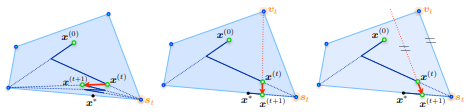
\includegraphics[width=\linewidth]{fig2.png}
% %   \caption{(left) The FW algorithm zig-zags when the solution $x$ lies on the
% % boundary. (middle) Adding the possibility of an away step attenuates this
% % problem. (right) As an alternative, a pairwise FW step.}
% %   \label{fig:Away steps}
% % \end{figure}

% To address this issue an improved variant of F-W named \textbf{Away-steps
% Frank-Wolfe} adds the possibility of moving away (by removing a fraction of) a
% maximizer of the $LMO_{\mathcal{S_{t}}}$ in the active set. While this slows
% down each iteration it should be noted that the added step is easier than
% $LMO_{\mathcal{A}}$ given that we maximize over a subset of $\mathcal{A}$.
% Furthermore, given that this variant converges linearly, the algorithm
% progresses in a fewer number of iterations in the descent direction, making it
% much faster than the original F-W.




% \subsubsection*{Randomized Away-step Frank-Wolfe}
% A crucial assumption in constructing the BCFW is whether the domain is
% block-separable. While this is true in the context of the structured SVM, this
% leaves out important cases such as $l_{1}$ constrained optimization (e.g. lasso
% type problems). \\
% Moreover, while being an improvement on the classical variant by being
% $n=\textit{size of the data}$ times cheaper per iteration, BCFW still converges
% at a sublinear rate unlike the Away-step FW.\\

% \textbf{The Randomized Away-steps Frank-Wolfe (RAWF)} finds a compromise between
% the two variants. By subsampling a $\eta\in(0,1]$ portion of the domain
% $\mathcal{A}$ in the $LMO$ and adding an away step at each iteration, we get a
% linear convergence rate with cheaper oracle calls than that of the original F-W.
% \subsubsection*{Convergence results}
% \textbf{Definition.}
% Let the \textit{away curvature} $C^{A}_{f}$ and the \textit{geometric strong convexity} constants be, respectively
% % 
% % \begin{aligned}
% %     &C^{A}_{f}= \underset{\underset{\underset{\gamma\in[0,1]}{y=x+\gamma(s-
% % x)}}{x,s,v\in\mathcal{M}}}{sup}\frac{2}{\gamma^{2}}\Big(f(y)- f(x)-
% % \gamma\langle \nabla f(x), s- v\rangle\Big)\\ &\mu^{A}_{f}=
% % \underset{x\in\matcal{M}}{\textit{inf}}\underset{\underset{\langle\nabla f(x),
% % x^{*}-x\rangle <
% % 0}{x^{*}\in\mathcal{M}}}{\textit{inf}}\frac{2}{\gamma^{A}(x,x^{*})^{2}}B_{f}(x,x^{*})\\
% % &\texit{where}\quad\gamma^{A}(x,x^{*})=\frac{\langle -\nabla f(x), x^{*}-
% % x\rangle}{\langle -\nabla f(x), s_{f}(x)- v_{f}(x)\rangle}\\
% % \end{aligned}
% % \end{equation*}
% And $s_{f}, v_{f}(x)$ are the FW atom and away atom respectively, starting from $x$.\\

% \textbf{Theorem.} Consider the set $\mathcal{M}=conv(\mathcal{A})$, with
% $\mathcal{A}$ a finite set of extreme atoms, adter $T$ iterations of RAFW, we
% have the following convergence rate
% 
% \begin{aligned}
%     &E\big[f(x_{T+1})\big]- f^{*}\leq \Big(f(x_{0})- f^{*}\Big).\Big(1- \eta^{2}\rho_{f}\Big)^{\textit{max}\{0,\lfloor\frac{T-s}{2}\rfloor\}}
% \end{aligned}
% \end{equation*}
% With $\rho_{f}=
% \frac{\mu^{A}_{f}}{4C^{A}_{f}},\quad\eta\frac{p}{|\mathcal{A}|}\quad$ and
% $\quad s=|S_{0}|$.\\

% \textbf{Proof sketch.} First we upper-bound $h_{t}=f(x_{t})- f^{*}$ by the
% pairwise dual gap $\tilde{g}_{t}=\langle \tilde{s}_{t}- v_{t}\rangle$, then we
% lower bound the progress $h_{t}- h_{t+1}$ by using the away curvature constant
% in similar way to the proof in (Lacoste-Julien \& Jaggi, 2015, Theorem
% 8).$\Box$\\ \\
% With the above theorem, we get
% 
% \begin{aligned}
%     &\underset{t\rightarrow \infty}{\textit{lim}} \frac{E f(x_{t+1})- f^{*}}{E f(x_{t})- f^{*}} \in \big(0,1\big)
% \end{aligned}
% \end{equation*}
% Thus proving a linear convergence rate for the Randomized Away-steps Frank-Wolfe.
% % \begin{algorithm}[tb]
% %    \caption{Randomized Away-steps Frank-Wolfe}
% %    \label{alg:example}
% \begin{algorithmic}
%     \STATE {Let $x_{0}=\sum_{v\in\mathcal{A}}\alpha^{(0)}_{v}$ with $s= |S_{0}|$, a subsampling parameter $1\leq p\leq |\mathcal{A}|$.}\\
%     \FOR {$t=0...T$}{
%         \STATE{Get $\mathcal{A}_{t}$ by sampling $min\{p,|\mathcal{A}\setminus S_{t}|\}$  elements uniformly from $|\mathcal{A}\setminus S_{t}|$}\\
%         \STATE {Compute $s_{t}= LMO(\nabla f(x), S_{t}\bigcup \mathcal{A}_{t})$}\\
%         \STATE {Let $d^{FW}_{t}= s_{t}- x_{t}$\quad\quad\textbf{RFW step}}\\
%         \STATE {Compute $v_{t}= LMO(-\nabla f(x), S_{t})$}\\
%         \STATE {Let $d^{A}_{t}= x_{t}- v_{t}$\quad\quad\quad\textbf{Away step}}\\
%         \STATE {\textbf{if} $\langle-\nabla f(x_{t}), d^{FW}_{t}\rangle\geq \langle-\nabla f(x_{t}), d^{A}_{t}\rangle$\quad\textbf{then}}\\ \STATE{\quad\quad\quad$d_{t}=d^{FW}_{t}$ and $\gamma^{max}=1$}\\
%         \STATE{\textbf{else}}\\
%         \STATE{\quad\quad\quad $d_{t}=d^{A}_{t}$ and $\gamma^{max}=\frac{\alpha^{(t)}_{v_{t}}}{1-\alpha^{(t)}_{v_{t}}}$}\\
%         \STATE{Let $x_{t+1}= x_{t}+ \gamma_{t}d_{t}$}\\
%         \STATE{Let $S_{t+1}= \{v\in\mathcal{A}\quad s.t.\quad \alpha^{(t)}_{v^{}_{t}} > 0$\}}\\
%     }
%     \ENDFOR
% \end{algorithmic}
% %\end{algorithm}

%%% Local Variables:
%%% mode: latex
%%% TeX-master: "mainProject"
%%% End:

% \clearpage
% In \citet{lacoste-julienBlockCoordinateFrankWolfeOptimization2013} 
% We define the \emph{linearize duality gap} for the k'th iterate as:
% \begin{equation}
%   g(\alpha^{k}) \triangleq \max_{s\in\mathcal{M}}\langle \alpha^{k}-s, \nabla f(\alpha^{k})\rangle
%   \label{eq:dualityGapDef}
% \end{equation}
% We
% \begin{align}
%     &f(s)\geq f(\alpha^{k})+ \langle \alpha^{k}-s, \nabla f(\alpha^{k})\rangle\\
%     &\Longrightarrow g(\alpha^{k})=
%       \min_{s\in\mathcal{M}}\langle \alpha^{k}-s, \nabla
%       f(\alpha^{k})\rangle \geq f(\alpha^{k})- f^{*}
% \end{align}
% We can thus see that the duality gap gives us a computable optimality guarantee. \\

% % \begin{definition}
% %   The curvature constant $C_{f}$ is given by the maximum relative deviation of
% %   the objective function f from its linear aaporximations, over the domain
% %   $\mathcal{M}$,
% % \end{definition}


% % \begin{align}
% %     &C_{f}= \underset{\underset{ \gamma\in[0,1],
% % y=x+\gamma(s-x)}{x,s\in\mathcal{M}}}{sup}\frac{2}{\gamma^{2}}\Big(f(y)- f(x)-
% % \langle y-x, \nabla f(x)\rangle\Big)
% % \end{align}
% % Intuitively, the curvature constant can be seen as a measure of how flat the
% % objective function is. For example, if the objective is linear, say $f(x)= ax+
% % b$ and $x\in[e,f]$ then $\nabla f(x)= a$ and the curvature constant is zero:
% % \begin{align}
% %     &C_{f}= \frac{2}{\gamma^{2}}\Big(ay+ b- ax- b +(-ay +ax)\Big)= 0
% % \end{align}
% % Moreover $s=\textit{argmin}_{s\in[e,f]}\langle s, a\rangle= \frac{e}{a}$. Hence
% % we reach the minimum in one F-W step. Thus, we can observe that for flatter
% % functions, that is with smaller curvature constants, Frank-Wolfe should converge
% % faster. 

% % \begin{theorem}
% %   The duality gap obtained in the $t^{th}$ iteraton of the Frank-Wolfe algorithm
% % satisfies
% % \begin{align}
% %     &g(x_{t})\leq 2\beta\frac{C_{f}}{t+2}(1+\delta)
% % \end{align}
% % Where $\beta= \frac{27}{8}$ and $\delta$ is the approximation error tolerated in
% % the $LMO$.
% % \end{theorem}


% %%% Local Variables:
% %%% mode: latex
% %%% TeX-master: "mainProject"
% %%% End:
\clearpage
\end{appendices}

\end{document}
